\documentclass[10pt,a4paper,danish]{article}
\usepackage[danish]{babel}
\usepackage[utf8]{inputenc}
\usepackage{amsmath}
\usepackage{amssymb}
\usepackage{listings}
\usepackage{fancyhdr}
\usepackage[hidelinks]{hyperref}
\usepackage{booktabs}
\usepackage{graphicx}
\usepackage{xfrac}
\usepackage[dot, autosize, outputdir="dotgraphs/"]{dot2texi}
\usepackage{tikz}
\usepackage{ulem}
\usepackage{lscape}
\usetikzlibrary{shapes}

\pagestyle{fancy}
\fancyhead{}
\fancyfoot{}
\rhead{\today}
\rfoot{\thepage}
\setlength\parskip{1em}
\setlength\parindent{1em}

%% Titel og forfatter
\title{ITS - aflevering 3}
\author{Søren Pilgård, 190689, vpb984\\
  René Løwe Jacobsen, 070192, vlx198}

%% Start dokumentet
\begin{document}

%% Vis titel
\maketitle
\newpage

%% Vis indholdsfortegnelse
\tableofcontents
\newpage

\section{Et online presserum}
Det problem, der springer i øjnene er, at koden giver mulighed for at åbne en
hvilken som helst fil på serveren, som den bruger webserveren kører på kan læse.
Dette kan gøres ved at ændre på GET-parametret pub og bruge ../ for at gå tilbage
mod roden på disken.

Et fix til dette problem kunne være at putte PHP applikationen i et jail, så det
ikke er muligt at komme udfra rodmappen for applikationen.
Man kunne også gøre sådan, at man i stedet for lavede linksne til filerne
direkte, så de ikke blev loaded af PHP.


\section{2}

\section{DDoS}
Vi har modtaget en log på 12.287.856 linjer som dækker alt trafik gennem
BIOChems firewall.
I loggen ses det hvordan et DDoSangreb starter på linje 1.876.657, kl. 13.53.00.
Angrebet slutter igen på linje 10.896.882 kl. 15.54.99 og varer dermed lige over 2
timer.
Der er dermed 9.020.225 linjers log for angrebet.

Som det ses i figur\ref{fig:ddos-pakker}, består angrebet af en stor mængde UDP
pakker sendt til BIOChems server udefra.

Et normalt UDPangreb går ud på at sende store mængder UDP pakker til en maskine.
Når en maskine modtager en UDP pakke, kontrolerer den om der kører et program
der lytter på den pågældende port, hvis ikke der gør, sendes en ICMP pakke som
svar på at intet kører der. UDP angrebet går således ud på at målet bruger
uforholdsvist meget tid på at finde ud af at ingen programmer lytter til en
given port og så sende en ICMP pakke til en addresse som højst sandsynligt ikke
er angriberens.

Som det ses i loggen er firewallen dog konfigureret til at afvise udp
forbindelser.
Det betyder at der i praksis ikke bliver behandlet nogle UDP pakker/sendt nogle
ICMP pakker. At angrebet lykkedes handler dermed om at man har sendt så meget
data at firewallen er kommet over sin kapacitet hvormed at man effektivt set har
blokeret for den normale brug af systemet.





Vi har målt aktiviteten som antal linjer per tidspunkt, dette er selvfølgelig
ikke et godt absolut mål da en almindelig tilgang til systemet generere 3
linjer, (en indkommen forbindelse, en forespørgsel og en nedpilning) hvorimod en
UDP pakke som angrebet består af kun generere én enkelt linje.
Det er dog fint til at vurdere den relative belastning af systemet.
På figur \ref{fig:ddos-all-activity}, \ref{fig:ddos-udp-activity} og
\ref{fig:ddos-non-udp-activity} ses det hvordan serveren bliver ramt.

En sjov detalje er hvordan der ca. hvert 20 minut under angrebet er et dyk i
pakker.
Man kunne forestille sig at det er firewallens netværkskort der forsøger at
komme tilbage på sporet ved at droppe en række pakker, hvilket ikke lykkes da
angrebet fortsætter.

\begin{landscape}
\begin{figure}[h!]\centering
\begin{verbatim}
May 20 13:53:00 130.255.254.1 %ASA-4-106023: Deny udp src outside:192.58.128.30/53 dst DMZ-1:www.biochem.dk/60847 by access-group "allowed-outside-inbound" [0x0, 0x0]
May 20 13:53:00 130.255.254.1 %ASA-4-106023: Deny udp src outside:192.58.128.30/53 dst DMZ-1:www.biochem.dk/44316 by access-group "allowed-outside-inbound" [0x0, 0x0]
May 20 13:53:00 130.255.254.1 %ASA-4-106023: Deny udp src outside:192.203.230.10/53 dst DMZ-1:www.biochem.dk/36044 by access-group "allowed-outside-inbound" [0x0, 0x0]
May 20 13:53:00 130.255.254.1 %ASA-4-106023: Deny udp src outside:192.112.36.4/53 dst DMZ-1:www.biochem.dk/39036 by access-group "allowed-outside-inbound" [0x0, 0x0]
May 20 13:53:00 130.255.254.1 %ASA-4-106023: Deny udp src outside:192.36.148.17/53 dst DMZ-1:www.biochem.dk/32700 by access-group "allowed-outside-inbound" [0x0, 0x0]
\end{verbatim}
\caption{De 5 første DDoS pakker.}
\label{fig:ddos-pakker}
\end{figure}
\end{landscape}

\begin{figure}[h!]
  \centering
  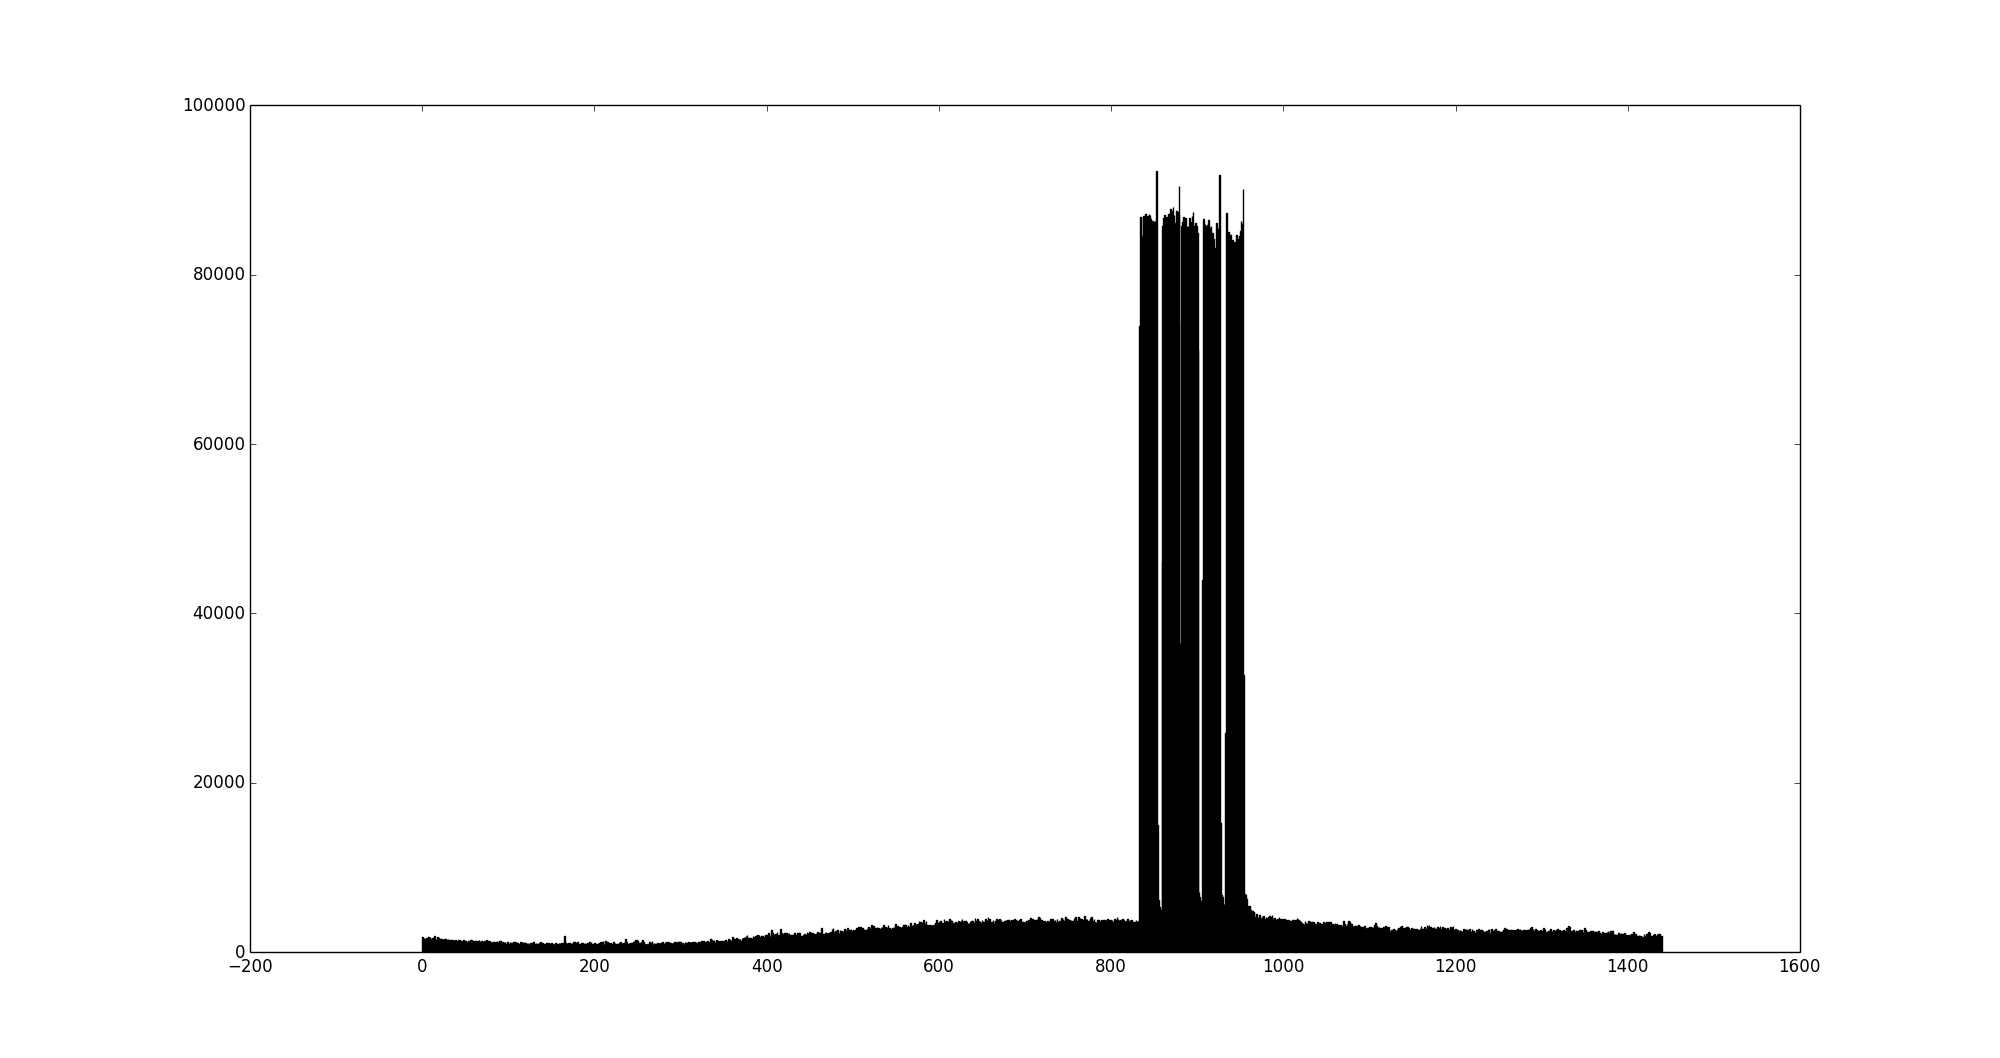
\includegraphics[width=\textwidth]{all-activity.png}
  \caption{Linjer i loggen pr. minut}
  \label{fig:ddos-all-activity}
\end{figure}

\begin{figure}[h!]
  \centering
  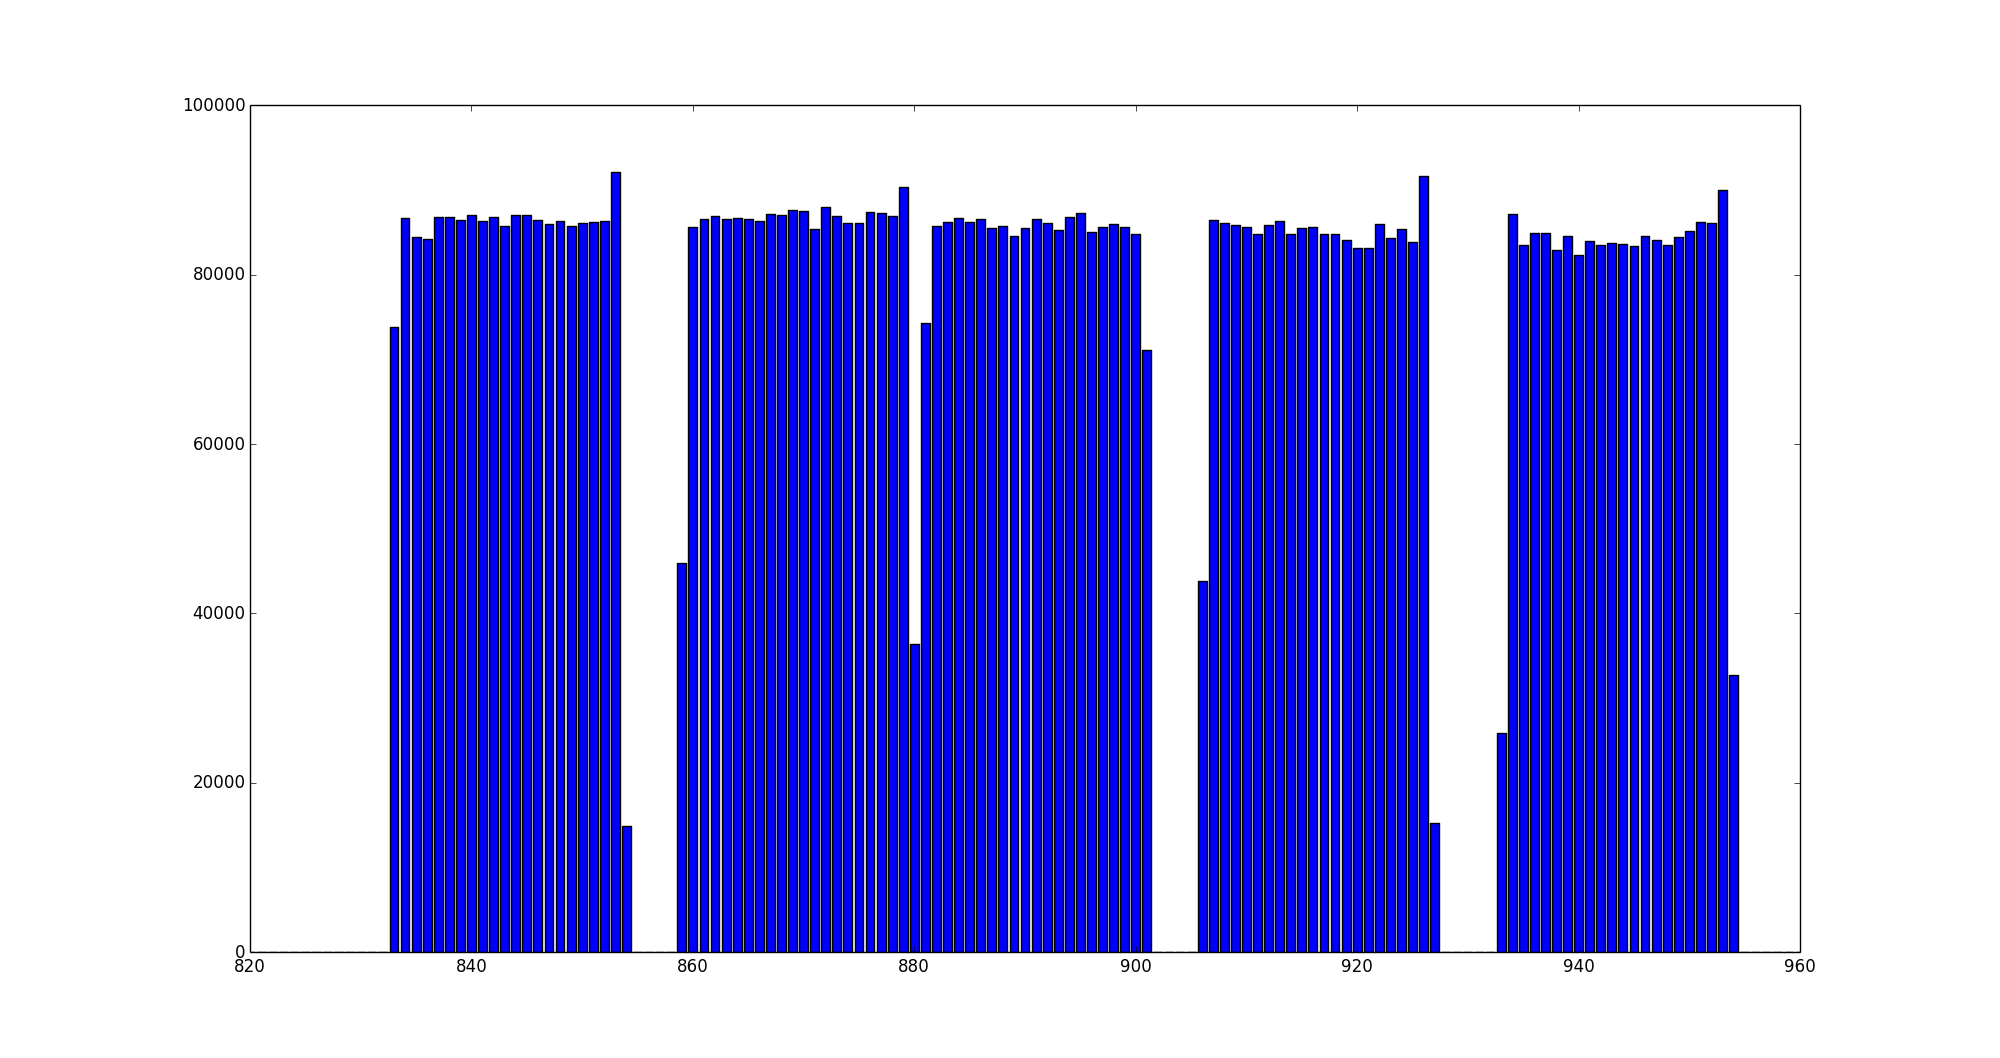
\includegraphics[width=\textwidth]{udp-activity.png}
  \caption{linjer i loggen der nævner udp pr. minut (startende fra minut 833 = kl. 13.53)}
  \label{fig:ddos-udp-activity}
\end{figure}

\begin{figure}[h!]
  \centering
  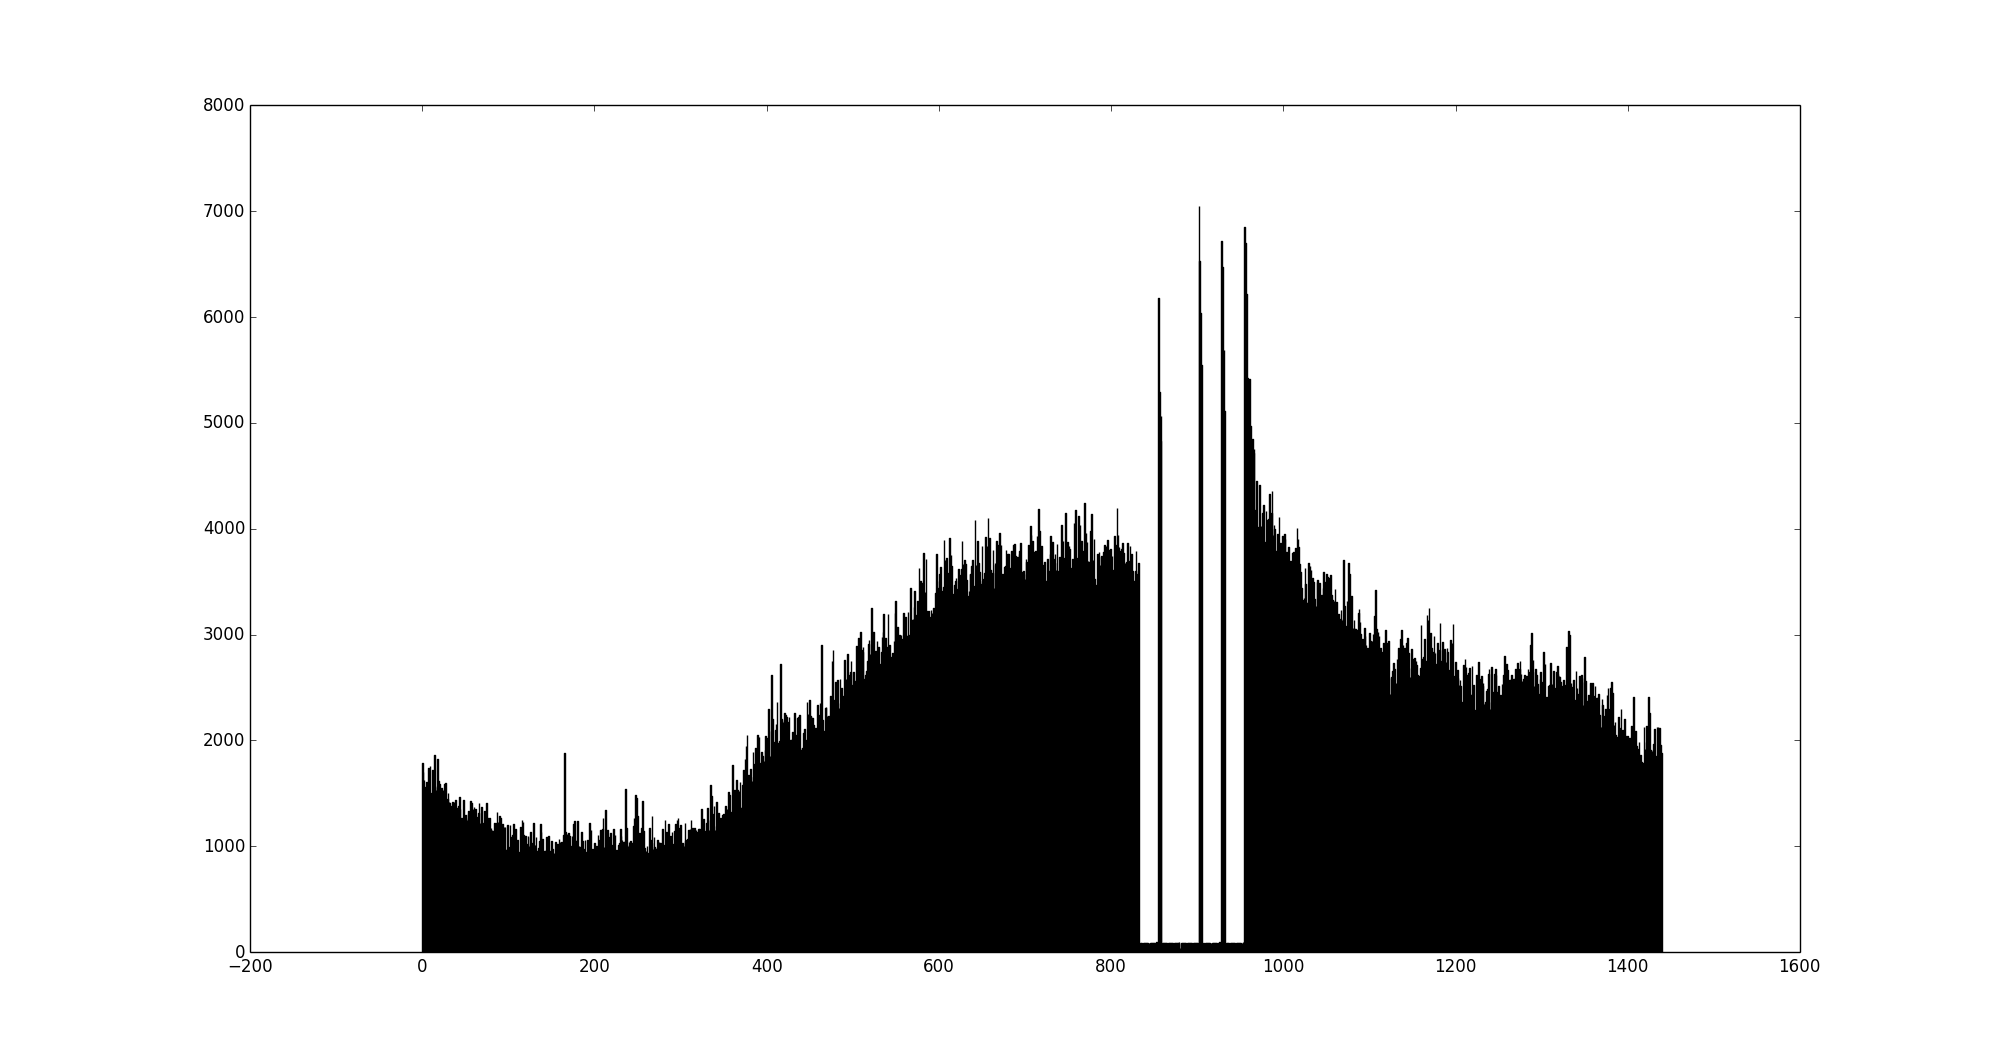
\includegraphics[width=\textwidth]{non-udp-activity.png}
  \caption{Linjer i loggen med andet end UDP pr. minut}
  \label{fig:ddos-non-udp-activity}
\end{figure}


\section{4}

\section{Litteraturliste}

\begin{thebibliography}{9}

\bibitem{cracking}
  \url{http://www.onlinehashcrack.com/how_to_crack_windows_passwords.php}, 21.
  maj 2014.

\bibitem{donotuse} Microsoft Developer Network,
  \url{http://msdn.microsoft.com/en-us/library/cc236715.aspx}

\bibitem{cracker1} \url{http://www.hashkiller.co.uk/ntlm-decrypter.aspx}
\bibitem{cracker2} \url{http://rainbowtables.it64.com/}

\end{thebibliography}


\end{document}
